\chapter{Observing Falling Filters}

	\begin{quotation}
		\textit{The ability to observe without evaluating is the highest form of intelligence.} \sourceatright{Jiddu Krishnamurti}
	\end{quotation}

While Mr.\ Krishnamuri may be making a stretch with his superlative, it remains true that observing without evaluating is essential for the creation of knowledge.
In our lives, we have bias (conceptions, self-constructed mental models) that we use as our lens to view the world.
These models are based on how each of us were socialized and on our subsequent experience.
To learn and create new knowledge, we must develop skill in observation.
In this lab, we will direct you to make detailed, careful quantitative observations, describe the patterns you find with mathematics, and finally make some wild guesses (``hypotheses'') about a more universal principle that explains this pattern that one could use to make predictions.
Due to time and brain constraints, we will not, in this lab, test those hypotheses.

\section*{Learning Goals}

 \begin{itemize}

  \item Become familiar with measurement, uncertainty, and writing lab reports.

  \item Learn how to conduct an observational experiment, including collecting data and analyzing the data to find and describe a pattern quantitatively.

  \item Use measurement uncertainty to describe physical quantities meaningfully.
  
  \item Format a lab report in a helpful way.
 \end{itemize}

\section*{The Scientific Cycle\protect\footnote{adapted from \cite{etkina_college_2014}}}

One way of describing science is the process of incrementally improving a shared model of how our universe works. In different fields of science, different methods and cycles are used, so there is no ``One True Scientific Method.'' One can still create a model for the process of science, and we describe here one such cycle, summarized in Figure~\ref{me:fig:isle}.

In this cycle, there are three types of experiments, each one representing a different stage of the scientific effort. One stage, often started when encountering a novel phenomenon, is the \textbf{observational experiment}. This is an experiment that consists of deciding what to observe and how to observe it, collecting data, finding a pattern, and brainstorming possible explanations for what is observed (also called ``hypotheses'').

Once one has some trial explanations, one can test one or more of those with a \textbf{testing experiment}. Here, one designs a new experimental procedure and uses each hypothesis to predict what will happen. Then the prediction is compared to the procedure's outcome. If they are different, then the hypothesis is judged to be not a helpful explanation for that phenomenon. If they are the same, then it is still helpful. Throughout this stage, one may make various assumptions that would need to be validated, as they can effect the prediction or outcome.

Once a hypothesis has been tested enough for people to find it useful, then it can be applied to solve practical problems, or to determine properties of particular situations, in an ``application experiment.''

%Astrophysics is an experimental science. To answer questions, astrophysicists do not just think and dream in their offices but constantly engage in experimental investigations. Astrophysicists use special measuring devices to observe phenomena (natural and planned), describe their observations (carefully record them using words, numbers, graphs, etc.), find repeating features called patterns (for example, the distance traveled by a falling object is directly proportional to the square of the time of flight), and then try to explain these patterns. By doing this, astrophysicists describe and answer the questions of ``why'' or ``how'' the phenomena happened and then deduce quantitative rules called mathematical models that explain the phenomena.

%However, a deduced explanation or a mathematical model is not automatically accepted as true. Every model needs to undergo careful testing. When astrophysicists test a model, they use the model to predict the outcomes of new experiments. As long as there is no experiment whose outcome is inconsistent with predictions made using the model, it is not disproved. However, a new experiment could be devised tomorrow whose outcome is not consistent with the prediction made using the model. The point is that there is no way to ``prove'' a model once and for all. At best, the model just hasn't been disproven yet.

%A simple example will help you understand some processes that physicists follow when they study the world. One model for the scientific process will also be described (there are other helpful models, and there is no one true ``scientific method''). Imagine that you walk into the house of your acquaintance Bob and see 10 tennis rackets of different quality and sizes. This is an \textbf{observational experiment}. During an observational experiment, a scientist collects data that seem important. Sometimes it is an accidental or unplanned experiment. The scientist has no prior expectation of the outcome. In this case, the number of tennis rackets and their quality and sizes represent the data. Having so many tennis rackets seems unusual to you, so you try to explain the data you collected (or, in other words, to explain why Bob has so many rackets) by devising several hypotheses. A \textbf{hypothesis} is an explanation that usually is based on some mechanism that is behind what is going on, or it can be a mathematical model describing the phenomenon. One hypothesis is that Bob has lots of children and they all play tennis. A second hypothesis is that Bob makes his living by fixing tennis rackets. A third hypothesis is that he is a thief who steals tennis rackets.

%How do you decide which hypothesis is correct? You may reason: if Bob has many children who play tennis, and I walk around the house checking the sizes of clothes that I find, then I will find clothes of different sizes. Checking the clothing sizes is a new experiment, called a \textbf{testing experiment}. A testing experiment is different from an observational experiment. In a testing experiment, a specific hypothesis is being ``put on trial.'' This hypothesis is used to construct a clear expectation of the outcome of the experiment. This clear expectation (based on the hypothesis being tested) is called a \textbf{prediction}. So you conduct the testing experiment by walking around the house checking the closets. You do find clothes of different sizes. This is the \textbf{outcome} of your testing experiment. Does it mean for absolute certain that Bob has the rackets because all of his children play tennis? No; he could still be a racket repairman or a thief. Therefore, if the outcome of the testing experiment matches the prediction based on your hypothesis, you cannot say that you proved the hypothesis. All you can say is that you failed to disprove it. However, if you walk around the house and do not find any children's clothes, you can say with more confidence that the number of rackets in the house is not due to Bob having lots of children who play tennis. Still, this conclusion would only be valid if you made an \textbf{assumption}: Bob's children live in the house and wear clothes of different sizes. Generally, in order to reject a hypothesis, you need to check the additional assumptions you made and determine if they are reasonable.

%Imagine you have rejected the first hypothesis (you didn't find any children's clothes). Next, you wish to test the hypothesis that Bob is a thief. This is your reasoning: \textit{If} Bob is a thief (the hypothesis), \textit{and} I walk around the house checking every drawer (the testing experiment), \textit{then} I will not find any receipts for the tennis rackets (the prediction). You perform the experiment and you find no receipts. Does it mean that Bob is a thief? He might just be a disorganized father of many children or a busy repairperson. However, if you find all the receipts, you can say with more confidence that he is not a thief (but he could still be a repairperson). Thus it is possible to disprove (rule out) a hypothesis, but it is not possible to prove it once and for all. The process that you went through to create and test your hypothesis is depicted in Figure~\ref{me:fig:isle}. At the end of your investigation you might be left with a hypothesis that you failed to disprove. As an astrophysicist you would now have some confidence in this hypothesis and start using it for practical applications, or \textbf{application experiments}.

\begin{figure}
	\centering
	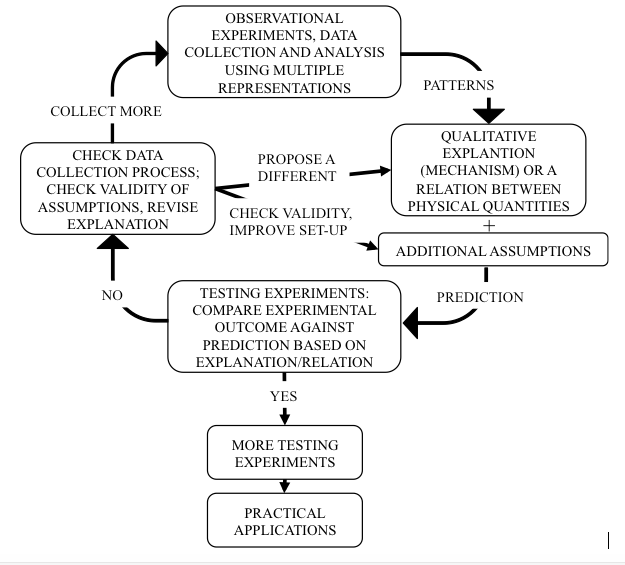
\includegraphics[width=0.7\textwidth]{measurement/islegraphic.png}
	\caption{A model of the process some scientists go through to create knowledge.\cite{etkina_millikan_2015}}\label{me:fig:isle}
\end{figure}

\section*{Observation experiment: Observing falling filters}

In today's lab, you will investigate the relationship between the size of coffee filters and how long it takes them to fall. In the first section, you will determine the size of the coffee filters. In the second, you will determine how long each take to fall, controlling for other variables, and then find a mathematical pattern that describes the relationship. Note that this lab does not include any hypothesis testing.

\begin{framed}
	\textbf{Self-assessment:} To help you improve your scientific abilities, we provide you with self-assessment rubrics.
	A rubric is a scoring system.
	Self-assessment is determining how well you performed a particular task.
	So, these self-assessment rubrics are designed to help you evaluate your performance while you are designing and performing your experiment.
	
	The complete set of rubrics is available in Appendix~\ref{cha:rubrics}.
	In each lab, your report will be assessed using Rubric F, found in Table~\ref{rubric:f}, as well as 5 additional rubric rows listed in that lab.
	Each week, read through these and use them to evaluate your work as you design and perform the experiment.
	Your instructor will use the same rubrics to determine part of your grade for the lab. In particular, each row will be worth 3 possible points (from ``Missing'' being 0 points to ``Adequate'' being 3 points).
\end{framed}	

\textbf{Rubrics to focus on during this experiment:} B5, B7, B8, F1, F2, G1, G2. See Appendix~\ref{cha:rubrics} for details.

\textbf{Available equipment:} several differently-sized coffee filters, meter stick, balance or scale, stopwatch, scratch paper%, camera (on your phone), Computer with ImageJ installed, string

You may want to \textbf{decide on roles} for each group member. Example roles include Facilitator (ensures time and group focus are efficiently used), Scribe (ensures work is recorded), Technician (oversees apparatus assembly, usage), Skeptic (ensures group is questioning itself). Note that each role is responsible for ensuring that the thing happens, rather than necessarily doing it themselves.

\subsection{How big are the filters?}

% DevNote: I decided to not make this a whole application experiment with 2 different methods, for the sake of time. I also removed image analysis with ImageJ, for the same reason. --bbarker, 2018-10-02

\textbf{Goal:} Find the cross-sectional area of each coffee filter and make a determination of that area, including uncertainty in that area, for use in the next section.
%In Stage 1 of the Barker X-Prize, each team has been tasked with determining precisely how big various objects are, including marbles, cotton balls, and coffee filters, including a detailed determination of their uncertainty of these measurements.
 
%\begin{framed}
%	ImageJ is an image analysis program that includes, among other things, the ability to measure lengths, angles, and areas in images, provided that you give it a scale for how long some reference object is in the image.
%\end{framed}

\begin{enumerate}
	\item Review Rubric G (Table~\ref{rubric:g}) and discuss any unclear expectations with your group and the instructor.
	
%	\item Discuss with your group what cross-sectional area means and why it might affect the fall time. Feel free to use your resources (books, internet, etc.) to do this.
	
	\item Brainstorm different methods you could use to determine the cross-sectional area. Feel free to play with the equipment as desired. Here are some things to consider:
	\begin{itemize}
		\item Will you measure the area directly, or will you measure something else and use that to calculate the area?
		
		\item With any method, you will probably make one or more assumptions about the shape of the filter. How valid are those assumptions?
		
		\item For each method you consider, there may be different sources of uncertainty --- the resolution of the measuring devices themselves, how you use them to measure, etc. If there is a source of random uncertainty, then you will need to take several measurements and use Appendix~\ref{unc:random} to determine the uncertainty. The decision of how many measurements to take is a trade-off between increasing precision (decreasing the uncertainty of the mean) and decreasing the time the measurement process takes.
		
		\item If you make a measurement and use that measurement in an equation to find the area, you will need to propagate uncertainty as described in Appendix~\ref{unc:sec:prop}.
	\end{itemize}
	% Come up with two independent methods for determining the cross-sectional area. The purpose is that if you make a mistake or wrong assumption in one method, then the method (hopefully) gives a different result than the other method. For discovering new things, this is one quantitative way of checking your work, since you don't have the answer ahead of time.

	\item Decide on your method and discuss it with an instructor before you begin. They will help increase the chances that your method will lead to successful results, or at least that the unhelpful path that you choose will take a short enough amount of time for you to change it when you discover it does not work. We want you to have productive failure that you have time to learn from.
	
	\item Write down an outline of your intended procedure. You might end up changing this as you go, but it is helpful to start with a plan and then change it, rather than having no plan at all.
	
	\item For your procedure, list the sources of uncertainty involved with each measurement. For each source, identify whether it is a random or instrumental uncertainty.
	
	\item Execute your procedure, including setup, data collection, calculation of area, uncertainty estimation and propagation.
	
	\begin{framed}
	At the end of this step, you should have a table of coffee filter cross-sectional areas, with uncertainties.
	\end{framed}
	
	\item Once you are done collecting this data, review your written procedure and correct it to match what you actually did, and ensure you have sketched any measurement setups, so you can include it in the lab report. In particular, ensure that you have enough written so you can demonstrate Rubric Rows F1, G1 and G2 in your report (see Tables~\ref{rubric:f} and \ref{rubric:g}).
	
\end{enumerate}
 
\subsection{How fast do the filters fall?}

\textbf{Goal:} Determine how long it takes each coffee filter to fall.

\begin{enumerate}
	\item Review Rubric B (Table~\ref{rubric:b}) and discuss any unclear expectations with your group and the instructor.
	
	\item Identify any variables (things that could change between measurements --- either between measurements of the same filter, or among different filters) that could affect the fall time other than the coffee filter's cross-sectional area. If there is controversy in the group, feel free to test what variables might affect that fall time.
	
	\item Since you are testing how the fall time is related to the filter's area, you should hold the other variables constant, so that they affect all the filters in the same way. For each variable identified in the previous step, decide how to keep that constant.
	
	\item Brainstorm different methods you could use to determine the time it takes for the filter to fall. Feel free to play with the equipment as desired. Here are some things to consider:
	\begin{itemize}
		
		\item Will you measure the fall time directly, or will you measure something else and use that to calculate the area?
		
		\item For each method you consider, there may be different sources of uncertainty --- the resolution of the measuring devices themselves, how you use them to measure, etc. If there is a source of random uncertainty, then you will need to take several measurements and use Appendix~\ref{unc:random} to determine the uncertainty.
		
		\item If you make a measurement and use that measurement in an equation to find the time, you will need to propagate uncertainty as described in Appendix~\ref{unc:sec:prop}.
	\end{itemize}
		
	\item Decide on your method and discuss it with an instructor before you begin. They will help increase the chances that your method will lead to successful results, or at least that the unhelpful path that you choose will take a short enough amount of time for you to change it when you discover it does not work. We want you to have productive failure that you have time to learn from.
	
	\item Write down an outline of your intended procedure. You might end up changing this as you go, but it is helpful to start with a plan and then change it, rather than having no plan at all.
	
	\item For your procedure, list the sources of uncertainty involved with each measurement. For each source, identify whether it is a random or instrumental uncertainty.
	
	\item Execute your procedure, including setup, data collection, calculation of area, uncertainty estimation and propagation.
	
	\begin{framed}
	At the end of this step, you should have a table of coffee filter cross-sectional areas, with uncertainties, with another column for fall time, with uncertainty in the fall time.
	\end{framed}
	
	\item Once you are done collecting this data, review your written procedure and correct it to match what you actually did, and ensure you have sketched any measurement setups, so you can include it in the lab report. In particular, ensure that you have enough written so you can demonstrate Rubric Rows B5, F1, G1 and G2 in your report (see Tables~\ref{rubric:b}, \ref{rubric:f}, and \ref{rubric:g}).
\end{enumerate}

Now that you have these measurements, it is time to find a pattern.

\subsection{Finding a pattern}

The penultimate step in an observational experiment is to find a pattern. Note that we are not explaining why this pattern is happening yet --- we are focusing on describing it first.

\textbf{Goal:} Find a pattern in the data and describe it mathematically.
\textbf{Available equipment:} Computer with spreadsheet software

\begin{enumerate}
	\item Use a plotting program, for example LibreOffice Calc or Microsoft Excel, to plot a graph of fall time vs. filter area. The independent variable should be on the horizontal axis. The axes should each be labeled with the quantity name and the unit in parentheses. For example, if you measured fall time in seconds, then the axis label should be something like ``fall time (s)''.
	
	\item In that graph, include also the uncertainty in each value. This usually involves right-clicking on a data point and selecting ``error bars''. Then you can highlight the column of cells that include the uncertainties.
	
	\item\label{filters:step:what-shape} Visually, discuss what shape the data points make. Speculate what kind of relationship you see. Is it proportional? Linear? Parabolic? Exponential? Logarithmic?
	
	\item Create a line of best fit (or ``trend line'') in the graph using the software. Choose the equation type to match what your group guessed in the previous step. If the line obviously does not match the data, try again with a different equation type. Quantitatively, the goodness of fit of a line (how close the line is to your data points) can be represented by the correlation coefficient, given as $r^2$ in the software. If $r^2 \gtrsim 0.8$, then the equation that you found describes the data fairly well. Record that equation and the $r^2$ (or RMSE if given).
	
	\item Make a final determination for describing in words the pattern found. If it applies, you should use one of the terms given in Step~\ref{filters:step:what-shape} in order to precisely describe the pattern.
	
	\item Review Rubric Rows B7 and B8 in Table~\ref{rubric:b} and ensure that you are demonstrating them here or have enough information to do so in your lab report.
\end{enumerate}

\subsection{Finishing up}

Before you leave lab, be sure that you have reviewed the 7 rubric rows that are being used to assess your report and that you are equipped to do as well on them as you would like to. The visuals that you should definitely have in your report are sketches of your measurement setups and a graph of fall time vs. filter area. You may want to have others as well, but those you will definitely need.

\subsection{Optional Fun Time Extra}

To extend the lab just a little bit and break out of the ``observational experiment'' frame, and to check to see if your mathematical pattern (line of best fit) is consistent with other physics principles, you can extrapolate down to zero cross-sectional area. As an optional part of the lab with no added benefit to your grade (but with perhaps glee for your inner scientist), you can do this.

Using your equation for the relationship between the two variables, predict the freefall time of an object with zero cross-sectional area. You can compare this with the theoretical value for this time $t$, given for an object that is falling from height $h$, with the strength of the local gravitational field $g = 9.8\:$m/s$^2$, with the following formula:
\begin{equation}
 t = \sqrt{\frac{2 h}{g}}
\end{equation}
How close did you get?

%Rationale:
%\begin{enumerate}
% \item want one experiment where students measure lengths and estimate uncertainties that are needed for data analysis. Lengths are intuitive things for students, no prior teaching needed. Then they see how those lengths compare to something else in a physics-y way. Then they graph it and decide what functions might describe them.
 
% \item falling and air resistance is good here. air resistance depends on cross sectional area, so length measurement. Data is not simple and obvious, but is instead messy, making pattern identification non-trivial, but still possible. Also cannot just use or look-up simple answers online -> authentic inquiry.
 
% \item so could do area vs. time to hit the floor. Can measure with video tracking, photogates, motion detector, stopwatch. need multiple sizes of coffee filters.
 
% \item Or position vs. time for different objects. This should give some interesting graphs, since objects can vary from no-meaningful-air-resistance to dominated-by-air-resistance constant. And the latter case should have an acceleration at the beginning, then constant, so it's more complicated. Must use video tracking or motion detection. So includes the skill of choosing with data to model. is there one function that works for all parts, or is there a transition between different situations?
 
% \item for video tracking, need to know how students can find framerate of videos they take, make sure it's easily imported to OSP Tracker.
%\end{enumerate}

\section{Post-lab survey}

To assist the instructors with understanding your experience in this lab, please also respond to the following questions on a scale from 1 to 7 (with 7 being the most)
\begin{enumerate}
	\item To what extent was the instructor's assistance needed?
	\item To what extent did you know what to do (goal of the task)?
	\item To what extent did you know how to do it?
	\item To what extent did you know how well you are doing?
	\item to what extent was the assignment challenging?
	\item To what extent did you feel knowledgeable and skillful during the lab?
	\item To what extent was the lab fun and interesting?
\end{enumerate}

\section{If in Stars class, also do this:}
\subsection{Remote Observing with the Stone Edge Observatory}

For two labs in this course, we will be taking observations remotely with the Stone Edge Observatory in Sonoma, California. We will use a queuing system to submit observations that are automatically scheduled and taken by the telescope. The data are then processed and typically available for analysis several days after they were obtained. To ensure that our data are taken and reduced in time for our in-lab analysis (which is subject to possible delays due to, e.g., the weather at the observing site), we will be submitting observations to the queue several weeks prior to lab in which they will be analyzed.

First, you will need to register for an account that will allow you to access the queue website. Make groups of two to three students so that there are no more than 5 groups in a section. Each group will use one member’s email to sign up for an account in the queuing system. A TA will be present to manually add each group. Each group will receive an email that will allow them to create an account. Since you will be sharing an account, be sure to share the account password (and obviously don't re-use one from another personal account).

Once you have an account, you will be able to log onto the queue and submit observations. To do so, go to the website \texttt{https://queue.stoneedgeobservatory.com/} and log-in with your group's credentials. Then navigate to \texttt{OBSERVATIONS} $\blacktriangleright$ \texttt{SUBMIT AN OBSERVATION}. This will take you to a form that allows you to input the specifics of your observation. These will be given to you for each lab.

\subsection{HR Diagram: Taking observations}
For this lab, each section will be taking observations of one of two star clusters --- NGC 869 and M15. You will then use this data to make color-magnitude diagrams of these clusters, which can then be compared with stellar evolution models to determine when these clusters formed. Table~\ref{hr_diagram_obs} lists the parameters for the observations to be taken in this lab - each section will be assigned a cluster, and each group in the section should submit one observation. Each group will then analyze their data in-lab, and will combine datasets. If there are fewer groups than observations, omit the longest-exposure observations.

\begin{table}
    \centering
    \caption{HR Diagram Lab Observations}
    \label{hr_diagram_obs}
    \begin{tabular}{|l|c|c|c|c|r|}
    \hline
    \textbf{Program} & \textbf{Target} & \textbf{Exp Time (s)} & \textbf{Exp Count} & \textbf{Bin}
         & \textbf{Filters} \\
    \hline
    General & M 15 & 1 & 1 & 2 & Dark, g', r'\\
    \hline
    '' & '' & 5 & '' & '' & '' \\
    \hline
    '' & '' & 10 & '' & '' & '' \\
    \hline
    '' & '' & 20 & '' & '' & '' \\
    \hline
    '' & '' & 40 & '' & '' & '' \\
    \hline
    '' & NGC 869 & 0.5 & '' & '' & ''\\
    \hline
    '' & '' & 1 & '' & '' & '' \\
    \hline
    '' & '' & 2 & '' & '' & '' \\
    \hline
    '' & '' & 5 & '' & '' & '' \\
    \hline
    '' & '' & 10 & '' & '' & '' \\
    \hline
    \end{tabular}
\end{table}